

\tikzset{every picture/.style={line width=0.75pt}} %set default line width to 0.75pt        

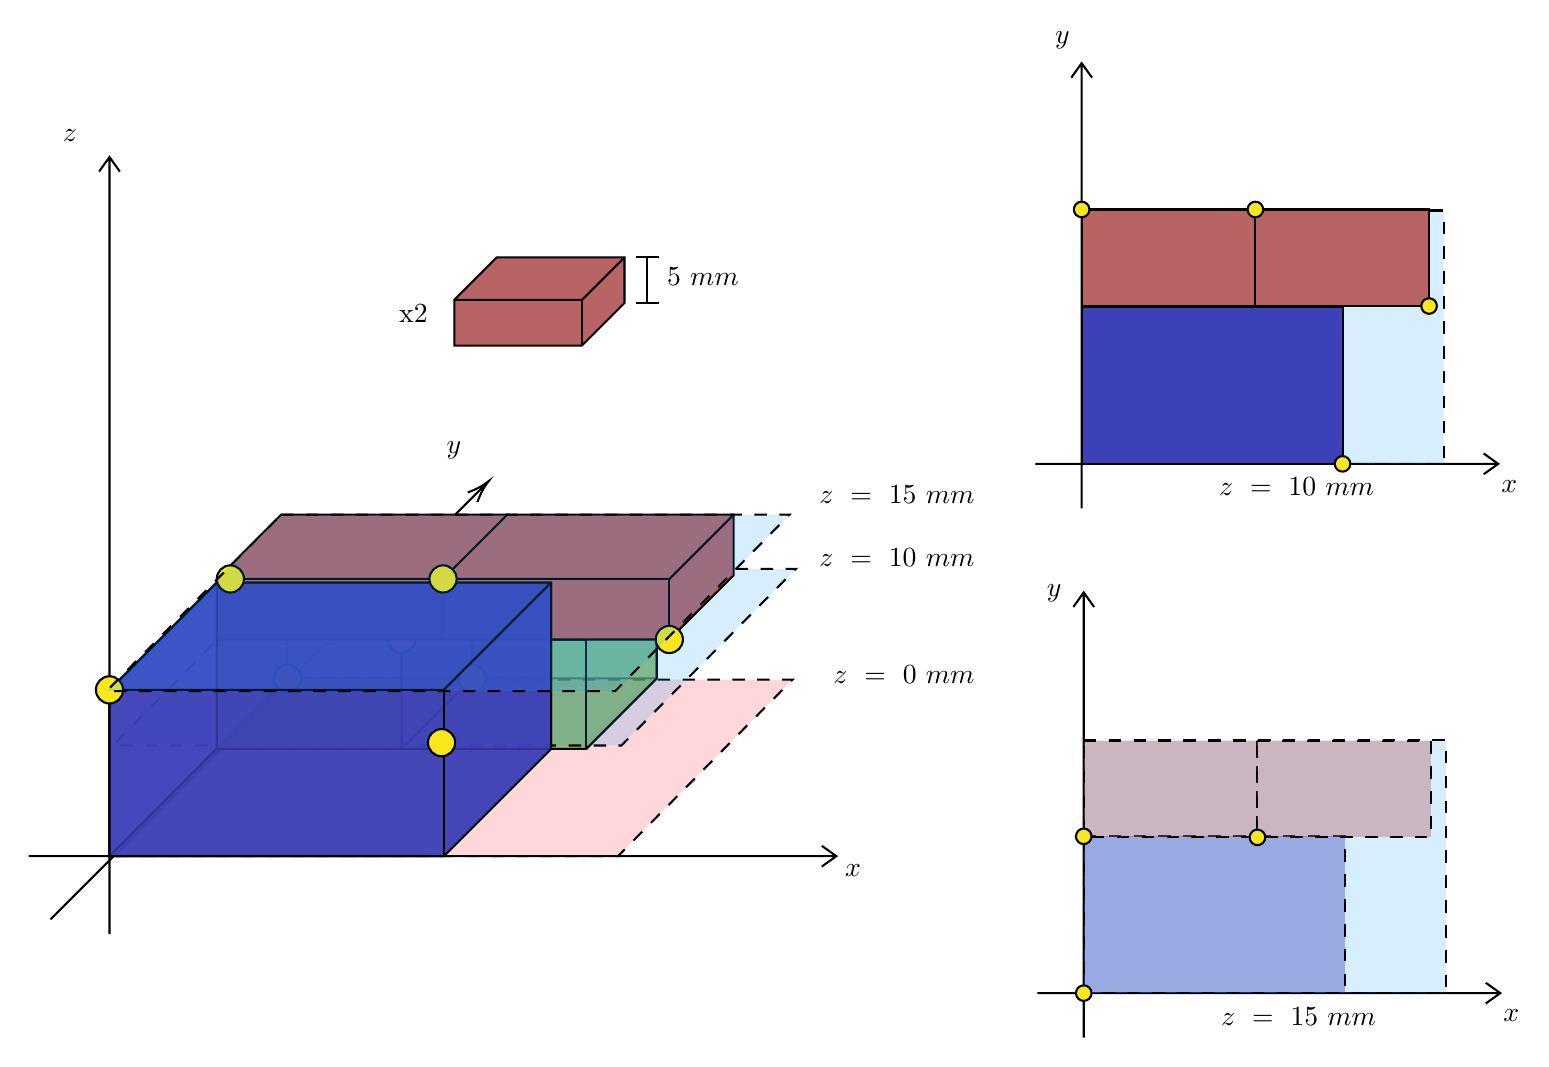
\begin{tikzpicture}[x=0.75pt,y=0.75pt,yscale=-1,xscale=1]
%uncomment if require: \path (0,536); %set diagram left start at 0, and has height of 536

%Shape: Cube [id:dp24118624821606238] 
\draw  [fill={rgb, 255:red, 130; green, 184; blue, 100 }  ,fill opacity=0.63 ] (380.59,330.87) -- (346.58,364.88) -- (257.6,364.88) -- (257.6,312.16) -- (291.6,278.15) -- (380.59,278.15) -- cycle ; \draw   (257.6,364.88) -- (291.6,330.87) -- (380.59,330.87) ; \draw   (291.6,330.87) -- (291.6,278.15) ;
%Shape: Parallelogram [id:dp818489623347525] 
\draw  [fill={rgb, 255:red, 255; green, 17; blue, 34 }  ,fill opacity=0.17 ][dash pattern={on 4.5pt off 4.5pt}] (201,331.5) -- (446,331.5) -- (361.91,416.57) -- (116.91,416.57) -- cycle ;
%Shape: Cube [id:dp029725286983864785] 
\draw  [fill={rgb, 255:red, 130; green, 184; blue, 100 }  ,fill opacity=0.63 ] (257.6,312.16) -- (291.6,278.15) -- (380.59,278.15) -- (380.59,330.87) -- (346.58,364.88) -- (257.6,364.88) -- cycle ; \draw   (380.59,278.15) -- (346.58,312.16) -- (257.6,312.16) ; \draw   (346.58,312.16) -- (346.58,364.88) ;
%Shape: Parallelogram [id:dp33144149017282] 
\draw  [fill={rgb, 255:red, 17; green, 154; blue, 255 }  ,fill opacity=0.17 ][dash pattern={on 4.5pt off 4.5pt}] (202.62,278.15) -- (447.62,278.15) -- (363.53,363.23) -- (118.53,363.23) -- cycle ;
%Shape: Axis 2D [id:dp7280305968897177] 
\draw  (78,416.57) -- (467.11,416.57)(116.91,79.72) -- (116.91,454) (460.11,411.57) -- (467.11,416.57) -- (460.11,421.57) (111.91,86.72) -- (116.91,79.72) -- (121.91,86.72)  ;
%Straight Lines [id:da37913853440794043] 
\draw    (88.47,447.02) -- (298.19,237.3) ;
\draw [shift={(299.6,235.89)}, rotate = 135] [color={rgb, 255:red, 0; green, 0; blue, 0 }  ][line width=0.75]    (10.93,-3.29) .. controls (6.95,-1.4) and (3.31,-0.3) .. (0,0) .. controls (3.31,0.3) and (6.95,1.4) .. (10.93,3.29)   ;
%Shape: Cube [id:dp43786688235829296] 
\draw  [fill={rgb, 255:red, 184; green, 100; blue, 100 }  ,fill opacity=1 ] (283.05,148.55) -- (303.55,128.05) -- (365.05,128.05) -- (365.05,150.05) -- (344.55,170.55) -- (283.05,170.55) -- cycle ; \draw   (365.05,128.05) -- (344.55,148.55) -- (283.05,148.55) ; \draw   (344.55,148.55) -- (344.55,170.55) ;
%Straight Lines [id:da5152098563828622] 
\draw    (376.05,128.05) -- (376.05,150.05) ;
\draw [shift={(376.05,150.05)}, rotate = 270] [color={rgb, 255:red, 0; green, 0; blue, 0 }  ][line width=0.75]    (0,5.59) -- (0,-5.59)   ;
\draw [shift={(376.05,128.05)}, rotate = 270] [color={rgb, 255:red, 0; green, 0; blue, 0 }  ][line width=0.75]    (0,5.59) -- (0,-5.59)   ;
%Shape: Cube [id:dp44715071573908904] 
\draw  [fill={rgb, 255:red, 130; green, 184; blue, 100 }  ,fill opacity=0.63 ] (291.6,330.87) -- (257.6,364.88) -- (168.61,364.88) -- (168.61,312.16) -- (202.62,278.15) -- (291.6,278.15) -- cycle ; \draw   (168.61,364.88) -- (202.62,330.87) -- (291.6,330.87) ; \draw   (202.62,330.87) -- (202.62,278.15) ;
%Shape: Cube [id:dp4497792783120459] 
\draw  [fill={rgb, 255:red, 130; green, 184; blue, 100 }  ,fill opacity=0.63 ] (168.61,312.16) -- (202.62,278.15) -- (291.6,278.15) -- (291.6,330.87) -- (257.6,364.88) -- (168.61,364.88) -- cycle ; \draw   (291.6,278.15) -- (257.6,312.16) -- (168.61,312.16) ; \draw   (257.6,312.16) -- (257.6,364.88) ;
%Shape: Ellipse [id:dp8025395959106266] 
\draw  [fill={rgb, 255:red, 248; green, 231; blue, 28 }  ,fill opacity=1 ] (196.07,330.87) .. controls (196.07,327.25) and (199,324.32) .. (202.62,324.32) .. controls (206.23,324.32) and (209.16,327.25) .. (209.16,330.87) .. controls (209.16,334.48) and (206.23,337.41) .. (202.62,337.41) .. controls (199,337.41) and (196.07,334.48) .. (196.07,330.87) -- cycle ;
%Shape: Axis 2D [id:dp6262269767988246] 
\draw  (564,482.55) -- (787,482.55)(586.3,289.5) -- (586.3,504) (780,477.55) -- (787,482.55) -- (780,487.55) (581.3,296.5) -- (586.3,289.5) -- (591.3,296.5)  ;
%Shape: Rectangle [id:dp7104361292217809] 
\draw  [fill={rgb, 255:red, 17; green, 154; blue, 255 }  ,fill opacity=0.17 ][dash pattern={on 4.5pt off 4.5pt}] (586.3,360.5) -- (761,360.5) -- (761,482.55) -- (586.3,482.55) -- cycle ;
%Shape: Rectangle [id:dp4551089431649423] 
\draw  [fill={rgb, 255:red, 61; green, 65; blue, 184 }  ,fill opacity=0.4 ][dash pattern={on 4.5pt off 4.5pt}] (586.3,407) -- (712,407) -- (712,482.55) -- (586.3,482.55) -- cycle ;
%Shape: Circle [id:dp4624770541343133] 
\draw  [fill={rgb, 255:red, 248; green, 231; blue, 28 }  ,fill opacity=1 ] (582.55,482.55) .. controls (582.55,480.48) and (584.23,478.8) .. (586.3,478.8) .. controls (588.37,478.8) and (590.05,480.48) .. (590.05,482.55) .. controls (590.05,484.62) and (588.37,486.3) .. (586.3,486.3) .. controls (584.23,486.3) and (582.55,484.62) .. (582.55,482.55) -- cycle ;
%Shape: Axis 2D [id:dp969470029295066] 
\draw  (563,227.55) -- (786,227.55)(585.3,34.5) -- (585.3,249) (779,222.55) -- (786,227.55) -- (779,232.55) (580.3,41.5) -- (585.3,34.5) -- (590.3,41.5)  ;
%Shape: Rectangle [id:dp4261055316386787] 
\draw  [fill={rgb, 255:red, 17; green, 154; blue, 255 }  ,fill opacity=0.17 ][dash pattern={on 4.5pt off 4.5pt}] (585.3,105.5) -- (760,105.5) -- (760,227.55) -- (585.3,227.55) -- cycle ;
%Shape: Rectangle [id:dp5378646202813674] 
\draw  [fill={rgb, 255:red, 61; green, 65; blue, 184 }  ,fill opacity=1 ] (585.3,152) -- (711,152) -- (711,227.55) -- (585.3,227.55) -- cycle ;
%Shape: Rectangle [id:dp8852671695477923] 
\draw  [fill={rgb, 255:red, 130; green, 184; blue, 100 }  ,fill opacity=0.4 ][dash pattern={on 4.5pt off 4.5pt}] (585.3,105.5) -- (655,105.5) -- (655,151.5) -- (585.3,151.5) -- cycle ;
%Shape: Circle [id:dp2270367067514596] 
\draw  [fill={rgb, 255:red, 248; green, 231; blue, 28 }  ,fill opacity=1 ] (707.25,227.55) .. controls (707.25,225.48) and (708.93,223.8) .. (711,223.8) .. controls (713.07,223.8) and (714.75,225.48) .. (714.75,227.55) .. controls (714.75,229.62) and (713.07,231.3) .. (711,231.3) .. controls (708.93,231.3) and (707.25,229.62) .. (707.25,227.55) -- cycle ;
%Shape: Rectangle [id:dp681624257096331] 
\draw  [fill={rgb, 255:red, 130; green, 184; blue, 100 }  ,fill opacity=0.4 ][dash pattern={on 4.5pt off 4.5pt}] (655,105.5) -- (724.7,105.5) -- (724.7,151.5) -- (655,151.5) -- cycle ;
%Shape: Ellipse [id:dp4533387898963953] 
\draw  [fill={rgb, 255:red, 248; green, 231; blue, 28 }  ,fill opacity=1 ] (285.06,330.87) .. controls (285.06,327.25) and (287.99,324.32) .. (291.6,324.32) .. controls (295.22,324.32) and (298.15,327.25) .. (298.15,330.87) .. controls (298.15,334.48) and (295.22,337.41) .. (291.6,337.41) .. controls (287.99,337.41) and (285.06,334.48) .. (285.06,330.87) -- cycle ;
%Shape: Ellipse [id:dp2258337282012488] 
\draw  [fill={rgb, 255:red, 248; green, 231; blue, 28 }  ,fill opacity=1 ] (251.05,312.16) .. controls (251.05,308.55) and (253.98,305.62) .. (257.6,305.62) .. controls (261.21,305.62) and (264.14,308.55) .. (264.14,312.16) .. controls (264.14,315.78) and (261.21,318.71) .. (257.6,318.71) .. controls (253.98,318.71) and (251.05,315.78) .. (251.05,312.16) -- cycle ;
%Shape: Ellipse [id:dp6988819335078928] 
\draw  [fill={rgb, 255:red, 248; green, 231; blue, 28 }  ,fill opacity=1 ] (270.37,361.87) .. controls (270.37,358.26) and (273.3,355.33) .. (276.91,355.33) .. controls (280.52,355.33) and (283.45,358.26) .. (283.45,361.87) .. controls (283.45,365.48) and (280.52,368.41) .. (276.91,368.41) .. controls (273.3,368.41) and (270.37,365.48) .. (270.37,361.87) -- cycle ;
%Shape: Cube [id:dp7385806895005637] 
\draw  [fill={rgb, 255:red, 184; green, 100; blue, 100 }  ,fill opacity=1 ] (168.61,283) -- (199.61,252) -- (308.63,252) -- (308.63,281.16) -- (277.63,312.16) -- (168.61,312.16) -- cycle ; \draw   (308.63,252) -- (277.63,283) -- (168.61,283) ; \draw   (277.63,283) -- (277.63,312.16) ;
%Shape: Cube [id:dp46845990607049726] 
\draw  [fill={rgb, 255:red, 184; green, 100; blue, 100 }  ,fill opacity=1 ] (277.63,283) -- (308.63,252) -- (417.65,252) -- (417.65,281.16) -- (386.65,312.16) -- (277.63,312.16) -- cycle ; \draw   (417.65,252) -- (386.65,283) -- (277.63,283) ; \draw   (386.65,283) -- (386.65,312.16) ;
%Shape: Cube [id:dp038868241472426956] 
\draw  [fill={rgb, 255:red, 61; green, 65; blue, 184 }  ,fill opacity=0.8 ] (329.7,364.88) -- (278,416.57) -- (116.91,416.57) -- (116.91,336.44) -- (168.61,284.75) -- (329.7,284.75) -- cycle ; \draw   (116.91,416.57) -- (168.61,364.88) -- (329.7,364.88) ; \draw   (168.61,364.88) -- (168.61,284.75) ;
%Shape: Ellipse [id:dp17174095369862896] 
\draw  [fill={rgb, 255:red, 248; green, 231; blue, 28 }  ,fill opacity=1 ] (380.11,312.16) .. controls (380.11,308.55) and (383.04,305.62) .. (386.65,305.62) .. controls (390.26,305.62) and (393.19,308.55) .. (393.19,312.16) .. controls (393.19,315.78) and (390.26,318.71) .. (386.65,318.71) .. controls (383.04,318.71) and (380.11,315.78) .. (380.11,312.16) -- cycle ;
%Shape: Cube [id:dp7592145851564649] 
\draw  [fill={rgb, 255:red, 61; green, 65; blue, 184 }  ,fill opacity=0.8 ] (116.91,336.44) -- (168.61,284.75) -- (329.7,284.75) -- (329.7,364.88) -- (278,416.57) -- (116.91,416.57) -- cycle ; \draw   (329.7,284.75) -- (278,336.44) -- (116.91,336.44) ; \draw   (278,336.44) -- (278,416.57) ;
%Shape: Ellipse [id:dp7845489096437979] 
\draw  [fill={rgb, 255:red, 248; green, 231; blue, 28 }  ,fill opacity=1 ] (110.37,336.44) .. controls (110.37,332.83) and (113.3,329.9) .. (116.91,329.9) .. controls (120.52,329.9) and (123.45,332.83) .. (123.45,336.44) .. controls (123.45,340.06) and (120.52,342.99) .. (116.91,342.99) .. controls (113.3,342.99) and (110.37,340.06) .. (110.37,336.44) -- cycle ;
%Shape: Ellipse [id:dp13625248726647632] 
\draw  [fill={rgb, 255:red, 248; green, 231; blue, 28 }  ,fill opacity=1 ] (168.61,283) .. controls (168.61,279.39) and (171.54,276.46) .. (175.15,276.46) .. controls (178.77,276.46) and (181.69,279.39) .. (181.69,283) .. controls (181.69,286.61) and (178.77,289.54) .. (175.15,289.54) .. controls (171.54,289.54) and (168.61,286.61) .. (168.61,283) -- cycle ;
%Shape: Ellipse [id:dp22786020311457056] 
\draw  [fill={rgb, 255:red, 248; green, 231; blue, 28 }  ,fill opacity=1 ] (271.09,283) .. controls (271.09,279.39) and (274.02,276.46) .. (277.63,276.46) .. controls (281.24,276.46) and (284.17,279.39) .. (284.17,283) .. controls (284.17,286.61) and (281.24,289.54) .. (277.63,289.54) .. controls (274.02,289.54) and (271.09,286.61) .. (271.09,283) -- cycle ;
%Shape: Parallelogram [id:dp2697731816540232] 
\draw  [fill={rgb, 255:red, 17; green, 154; blue, 255 }  ,fill opacity=0.17 ][dash pattern={on 4.5pt off 4.5pt}] (199.61,252) -- (444.61,252) -- (360.52,337.07) -- (115.52,337.07) -- cycle ;
%Shape: Rectangle [id:dp5173633377498139] 
\draw  [fill={rgb, 255:red, 184; green, 100; blue, 100 }  ,fill opacity=1 ] (585.3,105) -- (669,105) -- (669,151.5) -- (585.3,151.5) -- cycle ;
%Shape: Rectangle [id:dp6123569401126313] 
\draw  [fill={rgb, 255:red, 184; green, 100; blue, 100 }  ,fill opacity=1 ] (669,105) -- (752.7,105) -- (752.7,151.5) -- (669,151.5) -- cycle ;
%Shape: Circle [id:dp24876807610289275] 
\draw  [fill={rgb, 255:red, 248; green, 231; blue, 28 }  ,fill opacity=1 ] (748.95,151.5) .. controls (748.95,149.43) and (750.63,147.75) .. (752.7,147.75) .. controls (754.77,147.75) and (756.45,149.43) .. (756.45,151.5) .. controls (756.45,153.57) and (754.77,155.25) .. (752.7,155.25) .. controls (750.63,155.25) and (748.95,153.57) .. (748.95,151.5) -- cycle ;
%Shape: Circle [id:dp5040183450074549] 
\draw  [fill={rgb, 255:red, 248; green, 231; blue, 28 }  ,fill opacity=1 ] (665.25,105) .. controls (665.25,102.93) and (666.93,101.25) .. (669,101.25) .. controls (671.07,101.25) and (672.75,102.93) .. (672.75,105) .. controls (672.75,107.07) and (671.07,108.75) .. (669,108.75) .. controls (666.93,108.75) and (665.25,107.07) .. (665.25,105) -- cycle ;
%Shape: Circle [id:dp15069165887500435] 
\draw  [fill={rgb, 255:red, 248; green, 231; blue, 28 }  ,fill opacity=1 ] (581.55,105) .. controls (581.55,102.93) and (583.23,101.25) .. (585.3,101.25) .. controls (587.37,101.25) and (589.05,102.93) .. (589.05,105) .. controls (589.05,107.07) and (587.37,108.75) .. (585.3,108.75) .. controls (583.23,108.75) and (581.55,107.07) .. (581.55,105) -- cycle ;
%Shape: Rectangle [id:dp7396378678302288] 
\draw  [fill={rgb, 255:red, 184; green, 100; blue, 100 }  ,fill opacity=0.4 ][dash pattern={on 4.5pt off 4.5pt}] (586.3,361) -- (670,361) -- (670,407.5) -- (586.3,407.5) -- cycle ;
%Shape: Rectangle [id:dp5053870797116731] 
\draw  [fill={rgb, 255:red, 184; green, 100; blue, 100 }  ,fill opacity=0.4 ][dash pattern={on 4.5pt off 4.5pt}] (670,361) -- (753.7,361) -- (753.7,407.5) -- (670,407.5) -- cycle ;
%Shape: Circle [id:dp5616704740283756] 
\draw  [fill={rgb, 255:red, 248; green, 231; blue, 28 }  ,fill opacity=1 ] (582.55,407) .. controls (582.55,404.93) and (584.23,403.25) .. (586.3,403.25) .. controls (588.37,403.25) and (590.05,404.93) .. (590.05,407) .. controls (590.05,409.07) and (588.37,410.75) .. (586.3,410.75) .. controls (584.23,410.75) and (582.55,409.07) .. (582.55,407) -- cycle ;
%Shape: Circle [id:dp2597410649320595] 
\draw  [fill={rgb, 255:red, 248; green, 231; blue, 28 }  ,fill opacity=1 ] (666.25,407.5) .. controls (666.25,405.43) and (667.93,403.75) .. (670,403.75) .. controls (672.07,403.75) and (673.75,405.43) .. (673.75,407.5) .. controls (673.75,409.57) and (672.07,411.25) .. (670,411.25) .. controls (667.93,411.25) and (666.25,409.57) .. (666.25,407.5) -- cycle ;
%Shape: Ellipse [id:dp5241097716779531] 
\draw  [fill={rgb, 255:red, 248; green, 231; blue, 28 }  ,fill opacity=1 ] (270.37,361.87) .. controls (270.37,358.26) and (273.3,355.33) .. (276.91,355.33) .. controls (280.52,355.33) and (283.45,358.26) .. (283.45,361.87) .. controls (283.45,365.48) and (280.52,368.41) .. (276.91,368.41) .. controls (273.3,368.41) and (270.37,365.48) .. (270.37,361.87) -- cycle ;

% Text Node
\draw (464.19,323.16) node [anchor=north west][inner sep=0.75pt]    {$z\ =\ 0\ mm$};
% Text Node
\draw (277.9,215.2) node [anchor=north west][inner sep=0.75pt]    {$y$};
% Text Node
\draw (469.84,419.35) node [anchor=north west][inner sep=0.75pt]    {$x$};
% Text Node
\draw (92.94,65.14) node [anchor=north west][inner sep=0.75pt]    {$z$};
% Text Node
\draw (255,149.5) node [anchor=north west][inner sep=0.75pt]   [align=left] {x2};
% Text Node
\draw (384.05,131.45) node [anchor=north west][inner sep=0.75pt]    {$5\ mm$};
% Text Node
\draw (457.48,236.7) node [anchor=north west][inner sep=0.75pt]    {$z\ =\ 15\ mm$};
% Text Node
\draw (787,488.9) node [anchor=north west][inner sep=0.75pt]    {$x$};
% Text Node
\draw (571,17.9) node [anchor=north west][inner sep=0.75pt]    {$y$};
% Text Node
\draw (651,487.9) node [anchor=north west][inner sep=0.75pt]    {$z\ =\ 15\ mm$};
% Text Node
\draw (457.48,266.7) node [anchor=north west][inner sep=0.75pt]    {$z\ =\ 10\ mm$};
% Text Node
\draw (786,233.9) node [anchor=north west][inner sep=0.75pt]    {$x$};
% Text Node
\draw (650,232.9) node [anchor=north west][inner sep=0.75pt]    {$z\ =\ 10\ mm$};
% Text Node
\draw (567,284.4) node [anchor=north west][inner sep=0.75pt]    {$y$};


\end{tikzpicture}
